\documentclass[a4paper]{article}
\usepackage[utf8]{inputenc}
\usepackage[italian]{babel}
\usepackage{titling}
\usepackage{graphicx}
\usepackage{wrapfig}
\usepackage{float}
\usepackage{amsmath}
\usepackage{listings}
\usepackage[table,xcdraw]{xcolor}
\usepackage[numbers]{natbib}
\usepackage{amssymb}
\renewcommand{\bibfont}{\small}

\newcommand{\subtitle}[1]{%
	\posttitle{%
		\par\end{center}
	\begin{center}\large#1\end{center}
	\vskip0.5em}%
}

\begin{document}

%opening
\title{Studio della Stabilità dei Dischi di Accrescimento di Shakura \& Sunyaev}
\subtitle{Appunti}
\author{Riccardo Aurelio Gilardi}
\maketitle

\newpage
\tableofcontents
\newpage

\section{Introduzione}
Lo scopo di questa tesi vuole essere quello di riassumere ed approfondire le teorie sulla stabilità delle regioni interne dei dischi di accrescimento, nel contesto del modello introdotto da Shakura e Sunyaev nel loro articolo del 1973 ~\cite{ShakuraSunyaev1973}.

Anche se sarebbe interessante approfondire l'argomento, non considererò il caso dell'accrescimento a simmetria sferica, perché nonostante questo tipo di fenomeno abbia interessato i primi autori che si sono approcciati al tema dell'accrescimento (iniziando dagli studi di Zeldovich negli anni '40, ma continuando con gli studi sviluppatasi in seguito: Salpeter (1964), Lynden-Bell (1969), Schwartzmann (1971) e altri), nella letteratura si è dimostrato come si tratti di un meccanismo troppo poco efficente per essere rilevato, anche nel caso di corpi centrali molto massicci e compatti~\cite{PringleReesePacholczyk1973}.

Per mantenere una descrizione più semplice e meno dispersiva, ho deciso di lavorare seguendo l'esempio di molti autori, analizzando un sistema formato da una stella ordinaria e un buco nero. Questa scelta è guidata dal fatto che il materiale in accrescimento non risente di effetti legati alla relatività generale a distanze maggiori di tre volte il raggio di Scwartzchild del buco nero
\footnote{166FKR}
e, al contrario del caso di accrescimento intorno a una stella a neutroni, il sistema in accrescimento al buco nero non sarà interessato da fenomeni legati ai campi magnetici e alla torsione che essi possono applicare al materiale in accrescimento.

La scelta è anche giustificata dal fatto che, nonostante i buchi neri che fanno parte di sistemi binari siano meno semplici da osservare rispetto, per esempio, di quelli contenenti nane bianche, la loro estrema compattezza permette di apprezzare il comportamento del disco nelle sue regioni più interne.

Prima di parlare delle instabilità nei dischi, comincerò introducendo i concetti e le formule che descrivono un disco di accrescimento sottile, la fisica che ne governa lo stato stazionario e il meccanismo con cui si può arrivare alla formazione.

\newpage
\section{Accrescimento in sistemi binari}
	L'accrescimento è uno dei processi di conversione di massa in energia tra i più efficienti nell'universo, che si sviluppa in sistemi binari di cui almeno un membro è un corpo compatto: una nana bianca, una stella a neutroni o un buco nero.

	Tra le cause scatenanti del trasporto di materiale tra due membri di un sistema binario, sono particolarmente importanti il travalicamento da parte di uno dei membri del sistema del suo lobo di Roche o la cattura gravitazionale da parte del corpo compatto di venti stellari emessi dal suo compagno. Il primo di questi due processi è sicuramente meglio descritto e più semplice da trattare analiticamente e permette di dedurre delle informazioni interessanti sul processo dissipatovo che permette il trasporto del momento angolare. Una descrizione di questi processi permette di definire al meglio le ipotesi su cui si costruiscono i modelli di disco di accrescimento e permettono di fare osservazioni quantitative interessanti.
	
	Comunque è interessante sapere che la perdita di materiale tramite venti è molto comune e particolarmente importante quando l'accrescimento avviene con tassi superiori a quelli imposti dal limite di Eddington.
	
	\begin{equation}
		\dot{M}=\frac{4\pi GMm_pc^3}{\sigma_T \eta}
	\end{equation}

\subsection{Deflusso attraverso i Lobi di Roche}
	Edouard Roche ricavò la forma della struttura che ora prende il suo nome studiando l'orbita dei satelliti planetari. Lo fece descrivendo il moto di alcune particelle di test immerse in un potenziale gravitazionale generato da due corpi orbitanti intorno alla loro reciproca attrazione gravitazionale.
	
	La sua costruzione è essenziale e piuttosto elegante e si può ricavare partendo da poche semplici ipotesi, prima di calcolarne numericamente i parametri: la particella di test deve avere massa abbastanza piccola, al confronto con quella dei due corpi massicci, da non poterne influenzare in modo rilevante l'orbita; le orbite sono da considerarsi kepleriane e circolari, questo non è sempre vero in pratica, ma in generale le forze mareali tendono a rendere circolari orbite eccentriche in tempi scala molto minori di quelli caratteristici di un meccanismo di trasporto di materia; infine le masse sono da considerarsi condensate nel loro centro.
	
	Per descrivere qualsiasi flusso di gas tra i due corpi del sistema ha senso scrivere l'\textit{equazione di Eulero} in un sistema di riferimento co-rotante col sistema binario, con velocità angolare $\omega$ rispetto al sistema inerziale. Questo comporta la presenza nell'equazione di termini che tengano conto delle forze centrifughe e di quelle di Coriolis ($-2\omega\times\textbf{v}$), così che diventa:
	\begin{equation}
		\frac{\partial \textbf{v}}{\partial t}+(\textbf{v}\cdot\nabla)\textbf{v}=-\nabla\Phi_R-2\omega\times\textbf{v}-\frac{1}{\rho}\nabla P
	\end{equation}
	Con $\omega$ parallela al versore ortogonale al piano orbitale $\textbf{e}$:
	\begin{equation}
		\omega=\left[\frac{G(M_1+M_2)M_\odot}{a^3}\right]^{1/2}\textbf{e}
	\end{equation}
	e $\Phi_R$ il \textit{Potenziale di Roche}, che contiene i termini relativi all'attrazione gravitazionale e le forze centrifughe (ma non quelli relativi a Coriolis):
	\begin{equation}
		\Phi_R(\textbf{r})=-\frac{GM_1M_\odot}{\vert\textbf{r}-\textbf{r}_1\vert}-\frac{GM_2M_\odot}{\vert\textbf{r}-\textbf{r}_2\vert}-\frac{1}{2}(\omega\times\textbf{r})^2
	\end{equation}
	
	\begin{figure}[H]
		\centering
		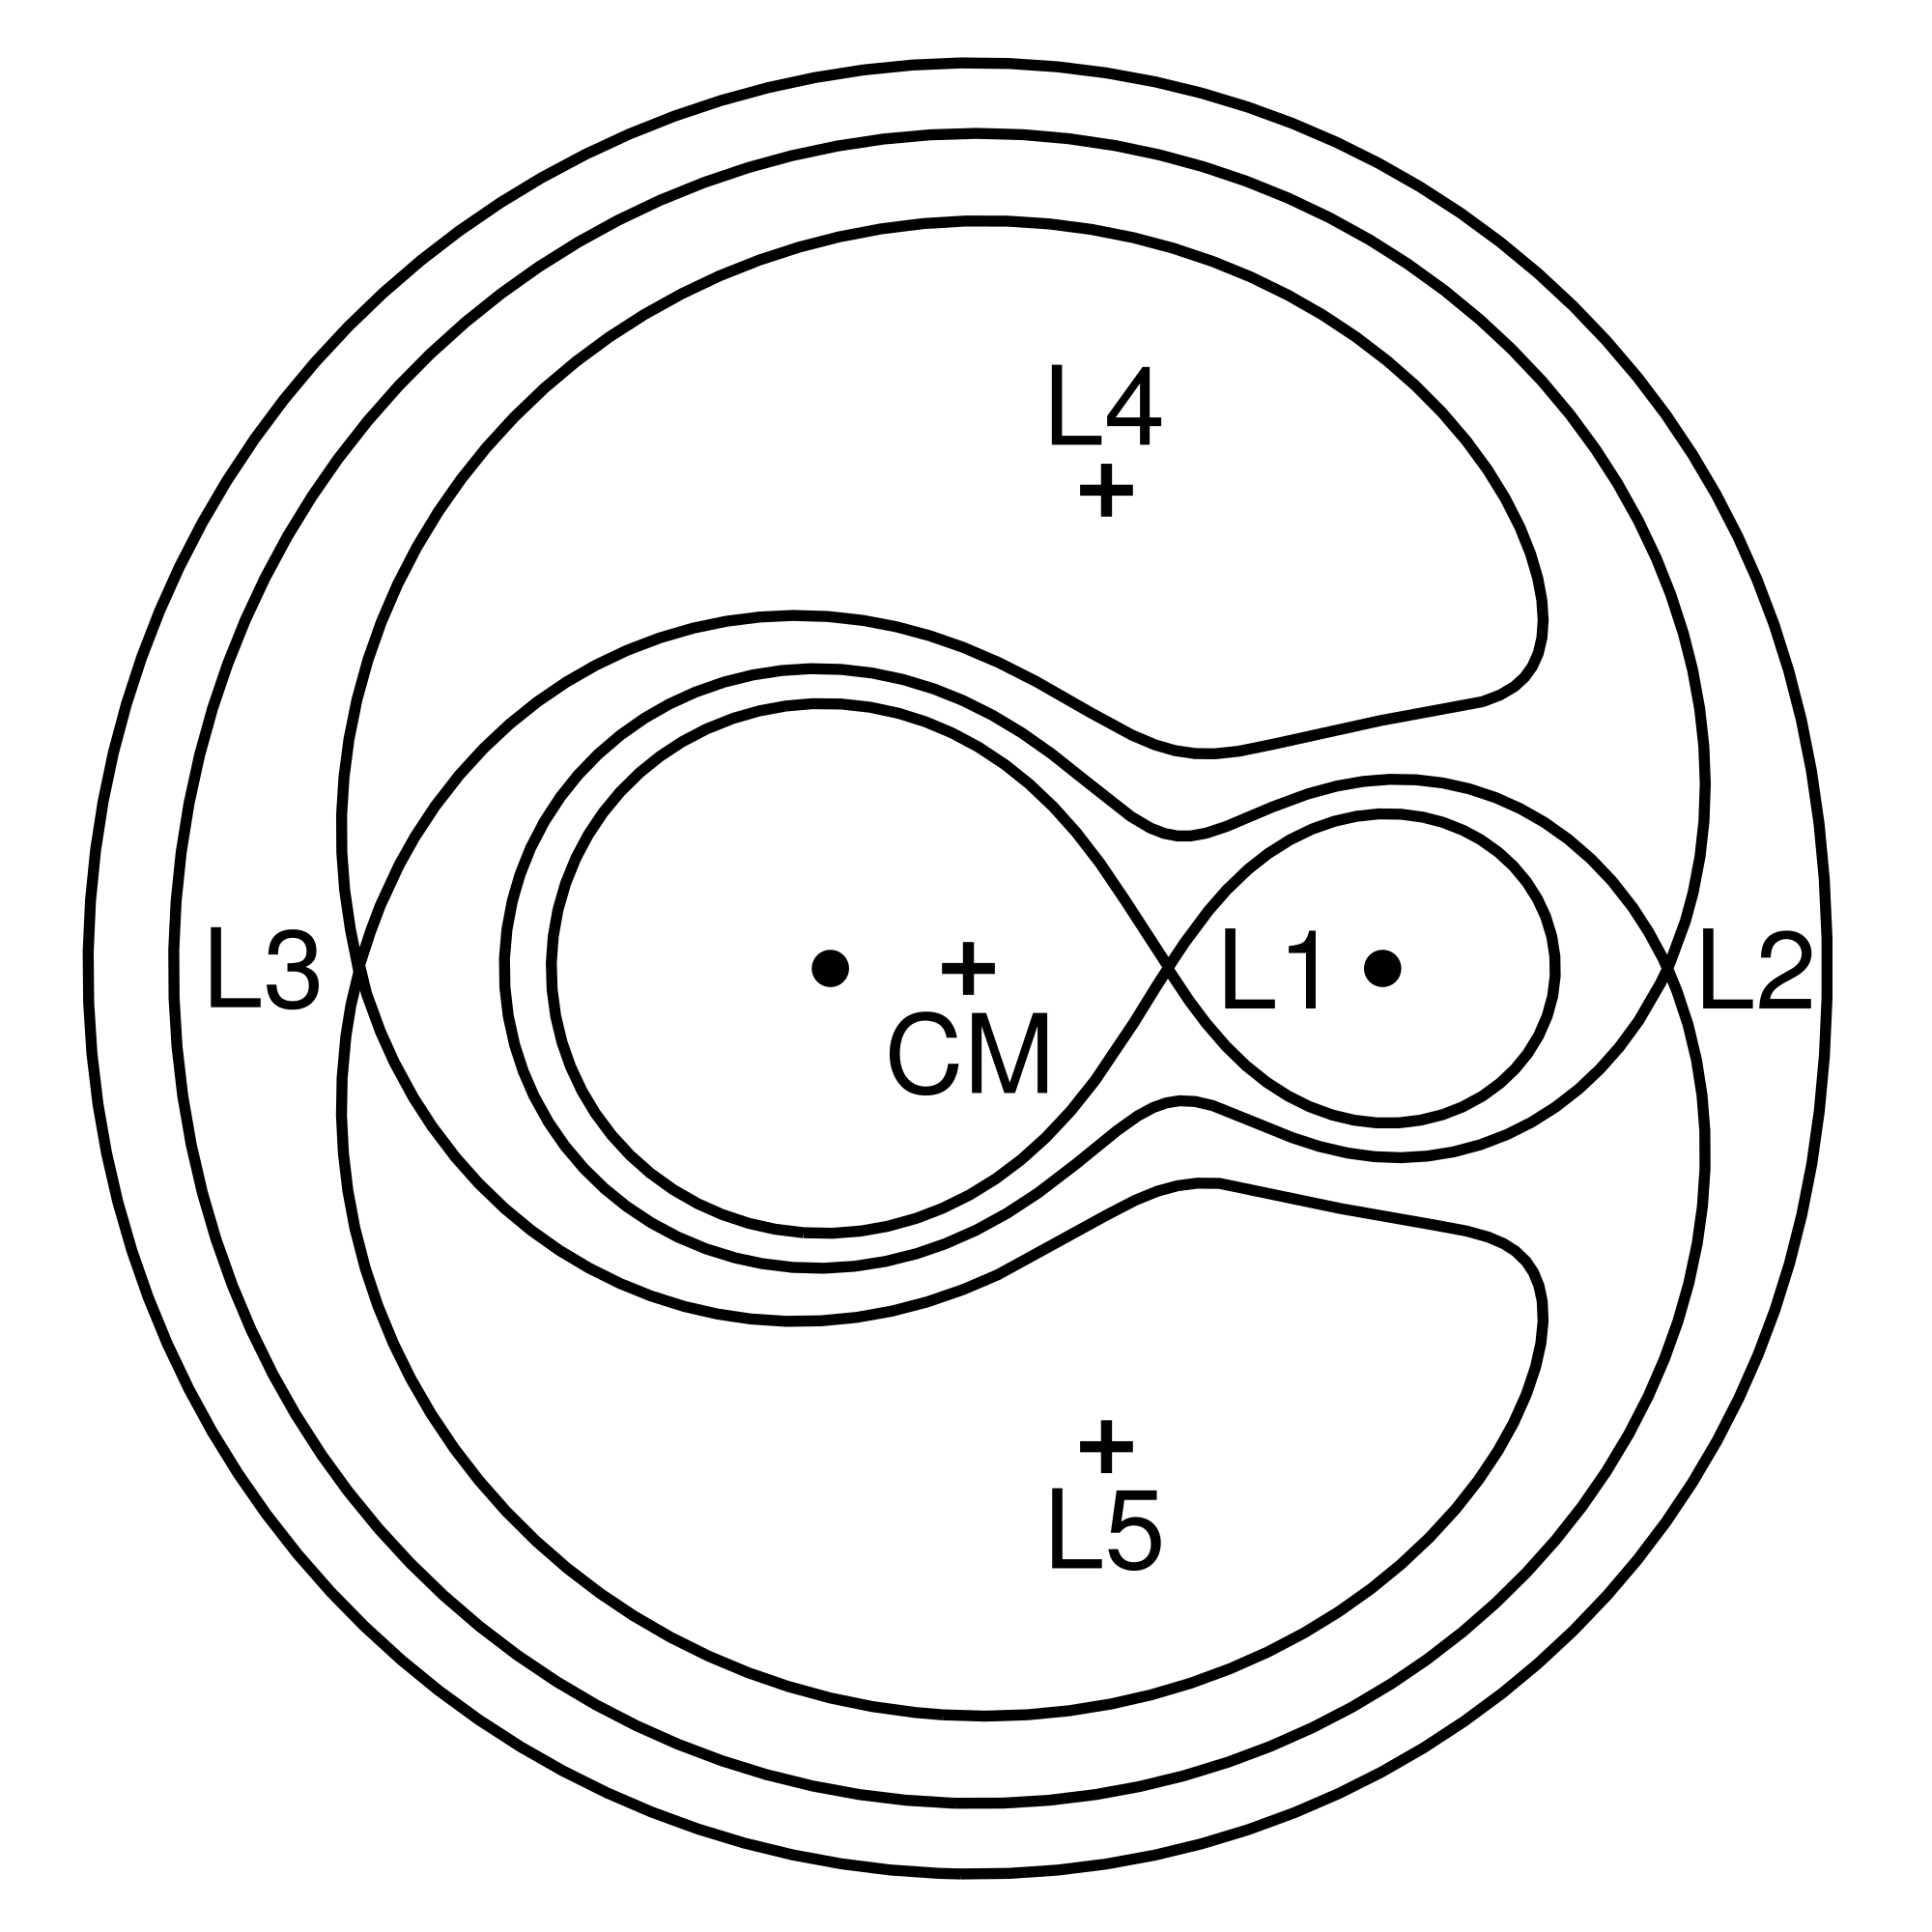
\includegraphics[width=0.6\linewidth]{RocheEquipotential}
		\caption{Una rappresentazione della sezione dei lobi e delle curve equipotenziali di $\Phi_R$. $L_1$ è il punto lagrangiano interno. Immagine da ~\cite{FrankKingRaineAccretionPower}}
		\label{fig:rocheequipotential}
	\end{figure}
	
	Le curve equipotenziali di $\Phi_R$ dipendono solo dal rapporto fra le masse $q=\frac{M_2}{M_1}$ e la loro scala dipende dalla distanza che le separa, $a$. Per $q\sim1$ i lobi saranno simmetrici, mentre per rapporti $q\ll1$ o $q>>1$ avranno volumi diversi.
	
	Per distanze sufficientemente alte, la forma delle curve equipotenziali corrisponde a quella di una singola massa $M=(M_1+M_2)M_\odot$, mentre a distanze brevi il potenziale è dominato da quello della stella più vicina. Le buche di potenziale centrate sulle posizioni dei due corpi $\textbf{r}_1$ e $\textbf{r}_2$, sono separate dalla cosiddetta \textit{superficie critica}.
	
	Il punto separatore dei due lobi, detto \textit{punto lagrangiano interno} è una sella per $\Phi_R$ tale che se del materiale in uno dei due lobi si trovasse in sua prossimità (magari a seguito dell'espansione della stella da cui proviene, che si ritroverà ad occupare tutto il volume del suo lobo), passerebbe attraverso lui verso il lobo della compagna, piuttosto che attraversare la superficie critica del potenziale.
	
	Si può trattare in maniera quantitativa la stima della geometria dei lobi e sul trasporto di materia, ricavando quindi la loro dipendenza da $q$ ed $a$. Qualcosa che è interessante osservare è che questi due termini varieranno nel tempo durante qualsiasi processo di accrescimento, comportando una contrazione del lobo del corpo che sta cedendo massa ed una riduzione del periodo orbitale del sistema, insieme alla riduzione della distanza tra i due corpi, dovuta al processo di trasferimento del momento angolare nel sistema.
	
	Si può dimostrare che, nell'ipotesi di accrescimento lento e totale $\dot{M}_1+\dot{M}_2=0$, il trasferimento di materia tra i due lobi si svolge nello stesso tempo scala con cui il momento angolare viene perso.
	
	Ipotizzando sia $M_2$, che chiameremo stella secondaria, a cedere materia a $M_1$, il nostro buco nero o primaria. Con $J$ momento angolare totale del sistema, abbiamo che:
	
	\begin{equation}
		-\frac{\dot{M}_2}{M_2}=\frac{-\dot{J}/J}{4/3-M_2/M_1}
	\end{equation}
	
	e analogamente si trova che

	\begin{equation}
		\frac{\dot{a}}{a}=2\frac{\dot{P}}{3P}=\frac{2\dot{J}/3J}{4/3-q}
	\end{equation}
	
\subsection{Formazione di un disco}
	Il trasporto di materia attraverso i lobi ne aumenta anche il momento angolare in quantità non indifferente, tanto da non permettere al materiale di essere accresciuto direttamente alla primaria, senza che qualche meccanismo gliene faccia trasportare la maggior parte.
	
	Se il periodo orbitale del sistema non è molto lungo, il lobo primario, ovvero quello a cui viene accresciuta la materia, la vedrà provenire dal punto lagrangiano con velocità quasi completamente ortogonale alla linea dei centri, che unisce le due masse. 
	
	Se definisco $b_1$ la distanza tra $M_1$ e $L_1$, posso approssimare il valore della componente istantaneamente ortogonale alla linea dei centri della velocità in un sistema di riferimento inerziale con
	\begin{equation}
		v_\perp\sim b_1\omega\sim 100\,M_1^{1/3}(1+q)^{1/3}P^{-1/3}_{day}\,km\,sec^{-1}
	\end{equation}  
	Mentre per la componente parallela, poiché immagino la forza che permette il passaggio tra i lobi della materia sia legata alla pressione, posso supporre valga
	\begin{equation}
		v_\parallel \lesssim c_{s}
	\end{equation}
	con $c_{s}$ velocità del suono nel lobo secondario, da cui proviene la materia. Poiché nel mezzo interstellare la temperatura ha valori $T\lesssim10^5\,K$ e poiché in generale per un gas vale $c_s\cong10(T/10^4\,K)^{1/2}km\,sec^{-1}$, deve essere $v_\parallel\lesssim10\,km\,sec^{-1}$
	
	Quindi in totale il moto del gas in ingresso al lobo primario deve essere supersonico. Questa condizione viene poi rinforzata dall'accelerazione che il materiale in accrescimento subirà per l'azione del campo gravitazionale del buco nero.

	\paragraph{Orbita del gas}	
	Si può dimostrare come le forze di pressione abbiano un effetto trascurabile sul materiale, che quindi si muoverà con orbita ballistica nel potenziale di Roche del corpo a cui sta accrescendo, come una particella di test. Inoltre il suo moto ellittico subirà una precessione dovuta all'effetto della presenza del corpo da cui proviene.
	
	Poiché $v_\parallel\sim c_s$ è molto minore delle velocità di free-fall che le particelle acquisirebbero nell'avvicinamento a $M_1$, le condizioni iniziale all'attraversamento di $L_1$ hanno un effetto praticamente irrilevante sulla loro orbita, che sarà quindi essenzialmente unica per ogni particella di test. Queste orbite dovranno comunque intersecarsi fra loro per via della precessione a cui sono soggette tutte singolarmente. Per un flusso continuo di gas, questo comporta la dissipazione di energia termica tramite degli urti (\textit{shock}) fra le particelle che lo formano. 
	
	Attraversato $L_1$, il gas in accrescimento si troverebbe, senza un meccanismo di dissipazione, a seguire l'orbita a potenziale minore per un dato momento angolare ($R_{circ}v_\phi(R_{circ})=b_1^2\omega$), ovvero un'orbita circolare, ad un certo raggio $R_{circ}$ e con velocità circolare
	\begin{equation}
		v_\phi(R_{circ})=\left(\frac{GM_1M_\odot}{R_{circ}}\right)^{1/2}
	\end{equation}
	
	E' possibile ricavare il valore del \textit{raggio di circolarizzazione} $R_{circ}$, utilizzando la formula del periodo della binaria $\omega=2\pi/P$ e si può ricavare tramite la computazione dei parametri dei lobi, come questo sia di un fattore $2\sim3$ più piccolo del raggio medio del lobo primario. Questo comporta che, a meno del caso in cui il raggio della primaria sia maggiore del raggio di circolarizzazione ($R_\star>R_{circ}$), la materia tenderebbe ad orbitare stabilmente nel lobo, una volta superata $L_1$.
	Non risulta interessante considerare l'eccezione sopracitata, poiché l'accrescimento è un processo tanto più efficente tanto più sono compatti gli oggetti intorno a cui avviene e se per una nana bianca realisticamente $R_{WD}\lesssim10^9\,cm$ normalmente ci si aspetta per il raggio di circularizzazione un valore $R_{circ}\gtrsim3.5\times10^9P_{hr}^{2/3}\,cm$.

	Un anello di materia dovrà necessariamente subire dei processi dissipativi, come degli urti, che convertiranno necessariamente parte dell'energia del moto orbitale delle particelle che lo formano in energia interna, ovvero calore. Parte di questa energia sarà irradiato, con una certa efficenza $\eta$ e quindi perso dal gas, costringendo le sue particelle interessate dalla dissipazione ad avvicinarsi alla primaria (nell'ipotesi in cui risentano del solo potenzile gravitazionale del corpo massiccio). 
	Affinché sia conservato il momento angolare nel disco, parte del momento delle particelle che si stanno avvicinando al corpo massiccio dovrà essere trasportato verso l'esterno. Il tempo di redistribuzione del momento angolare è maggiore sia dei tempi scala di raffreddamento radiativo $t_{rad}$ che di quello orbitale (dinamico) $t_{din}$. 
	
	Quindi parte del gas che orbitava sul raggio di circularizzazione, perdendo energia e trasportando momento angolare, spiraleggerà lentamente verso la primaria, costretto in una serie di orbite approssimamente circolari, nella configurazione cosiddetta di \textbf{disco di accrescimento}. 	In assenza di torsioni esterne, mi aspetto che le particelle esterne del disco, a cui viene trasferito momento, debbano spiraleggiare verso l'esterno a raggi maggiori di quelli di circularizzazione, fino a a una distanza tale per cui qualche meccanismo non gli impedisca di allontanarsi oltre\footnote{In realtà poiché il \textit{momento angolare specifico} $h$ per materia che orbita ad un raggio $R$ vale $h=R^2\Omega\propto R^{1/2}$ e quindi tende all'inifinito per raggi infiniti, la materia tenderà definitivamente a dirigersi verso il centro del disco, con il momento che tenderà ad allontanarsi a distanze sempre maggiori.}.
		
\subsection{Processi Dissipativi}
	Per un elemento di gas di massa $m$, che stia raggiungendo l'ultima orbita stabile (Innermost Stable Circular Orbit) intorno al buco nero, l'energia di legame varrà $E=\frac{1}{2}\frac{GMm}{R_\star}$. Considerando il valore di questa energia come trascurabile alla distanza da cui provengono, posso dire che la luminosità totale del disco dovrà valere
	
	\begin{equation}
		L_{disc}=\frac{GM\dot{M}}{2R_\star}=\frac{1}{2}L_{acc}
	\end{equation}

	Questo comporta che se metà dell'energia viene irradiata dalla materia che si muove verso l'ISCO, l'altra metà dovrà essere irradiata tutta nelle regioni più interne. Inoltre se considero che il momento angolare per raggio vale $R^2\Omega(R)\propto R^{1/2}$ e che $R_{ISCO}\ll R_{circ}$, il gas che forma il disco dovrà perdere quasi completamente il suo momento nella discesa verso la primaria.
	
	Nel contesto dei dischi di accrescimento, strutture gassose con una rotazione differenziale rispetto al raggio di particelle con velocità circa ortogonale alla direzione radiale, posso supporre che il meccanismo di trasporto del momento angolare e di dissipazione dell'energia in calore sia legato alla \textit{tensione viscosa di taglio} che si esercita fra strati diversi del disco.
	
	Si può capire come avvenga il trasporto di momento angolare per dissipazione viscosa considerando per esempio due strati successivi del disco di uno spessore arbitrariamente piccolo $\lambda$, separate da una superficie a che si trova a distanza $R$ dal centro del buco nero. Elementi del fluido che forma il disco, muovendosi caoticamente, potranno continuamente venire scambiati tra i due strati con velocità $\tilde{v}$. Questi elementi percorreranno in media una distanza $\lambda$ prima di interagire con elementi dello strato che hanno raggiunto e poiché la loro velocità dipendeva dal raggio a cui sono partiti, dopo una serie di scambi, ci sarà un \textit{trasporto netto di momento angolare} tra i due strati. Questo senza un trasporto netto di materia, per simmetria.
	
	\paragraph{Forma della viscosità}	
	Al momento non siamo ancora in grado di dare prescrizioni fisiche per la stima dei valori di $\lambda$ e $\tilde{v}$, così strettamente legati al significato fisico della dissipazione viscosa che agisce nel disco. Risultati moderni collegano la viscosità a processi magnetici, come suggerito da Balbus e Hawley nel 1991, ma non esiste ancora una risposta certa o esaustiva a riguardo. 
	
	Si dimostra che la densità di forza viscosa di taglio vale
	\begin{equation}
		f_{visc,taglio}\sim\rho\lambda\tilde{v}\frac{\partial^2v_\phi}{\partial R^2}\sim\rho\lambda\tilde{v}\frac{v_\phi}{R^2}
	\end{equation}
	Questo ci permette di ricavare un valore per il \textit{termine di Reynolds}, che stima l'importanza dinamica del termine viscoso rispetto a quello inerziale (ovvero $\rho(\partial\textbf{v}/\partial t+(\textbf{v}\cdot\nabla)\textbf{v})$, estratto dall'equazione di Eulero)
	\begin{equation}
		Re\sim\frac{v_\phi^2/R}{\lambda\tilde{v}v_\phi/R^2}=\frac{Rv_\phi}{\lambda\tilde{v}}
	\end{equation}
	Quindi possiamo dimostrare che la viscosità che permette l'accrescimento non è semplicemente quella classicamente legata ad un gas, per cui sarebbero $\lambda\sim\lambda_d$ \textit{tempo di deflessione} delle particelle del gas e $\tilde{v}\sim c_s$ velocità del suono, poiché in questo caso, utilizzando risultati della fluidodinamica, troviamo che $Re_{mol}\gtrsim10^4$ in regioni interne a un tipico disco di accrescimento. Questo valore iplicherebbe una irrilevanza estrema del termine viscoso rispetto a quello inerziale nel disco, dimostrando che la "viscosità molecolare" non può essere responsabile del trasporto.
	
	Poiché si è dimostrata sperimentalmente l'esistenza di un \textit{numero di Reynold critico} oltre cui il moto del gas diventa turbolento, con grandi variazioni di velocità in grande e piccola scala, si potrebbe supporre che anche nei dischi di accrescimento il processo principale di redistribuzione del momento angolare sia un moto turbolento, anche se non è stato dimostrato.
	La viscosità in questo tipo di sistema dipenderebbe da una lunghezza caratteristica dei vortici pi grandi, che ci aspettiamo non poter superare l'altezza del disco $\lambda_{turb}\lesssim H$ e da una velocità degli stessi vortici che ci aspettiamo essere subsonica $v_{turb}\lesssim c_s$, tali per cui $\nu_{turb}\sim \lambda_{turb}v_{turb}$.
	Poiché non siamo ancora in grado di descrivere matematicamente un moto turbolento, né capiamo appieno i meccanismi fisici che ne regolerebbero l'intesità, si è dimostrato utile, in un approccio semi-empirico all'analisi dei dischi, parametrizzare la viscosità con
	\begin{equation}
		\nu=\alpha c_s H
	\end{equation}
	Questa è la cosiddetta \textit{condizione $\alpha$ di Shakura e Sunyaev}, con $\alpha\lesssim 1$ adimensionale: una parametrizzazione utile per la costruzione di un modello di disco, che riesce a sintetizzare la nostra ignoranza sulla natura della viscosità, che non ci permette di avere un modello deterministico di disco.

	\paragraph{Momento torcente, densità superficiale ed energia dissipata}
	Una frazione di fluido dallo strato più interno trasporterà in media un momento $L(R+\lambda/2)$, mentre una dallo strato più esterno trasporterà in media $L(R-\lambda/2)$. Questo trasporto netto si traduce in una \textit{torsione del disco interno su quello esterno}.
	
	Se i due strati hanno densità $\rho(R)$ e altezza $H(R)$, ci sarà un trasporto di materia netto nell'ordine di $H\rho\tilde{v}$, per un osservatore co-rotante con il fluido che si trovi sulla superficie di separazione, il \textit{momento torcente medio} che si esercitano reciprocamente, per unità di angolo e al primo ordine in $\lambda$
	\begin{equation*}
		-\rho\tilde{v} H\lambda R^2\frac{d\Omega}{dr}
	\end{equation*}
	E per il nostro sistema di dischi concentrici, definendo la \textit{densità superficiale} $\Sigma=H\rho$ e il \textit{coefficente di viscosità cinematica} $\nu\sim\lambda\tilde{v}$, possiamo scrivere il \textit{momento torcente} esercitato dal disco esterno su quello interno come
	\begin{equation}
		G(R)=2\pi R\nu\Sigma R^2\frac{d\Omega}{dr}
	\end{equation}
	Si può apprezzare l'efficacia di questa formula nel descrivere l'accrescimento notando come si annulla nel caso di una rotazione rigida $\Omega'=\frac{d\Omega}{dr}=0$ ed è negativa nel caso in cui la velocità angolare decresca allontanandosi dal centro del disco, comportando quindi il trasporto del momento angolare dagli strati più interni verso quelli più esterni, con il conseguente spiraleggiare verso l'interno del gas.
	
	Dalla conservazione del momento angolare per gli anelli possiamo ricavare un equazione differenziale in R che dipenda dall'evoluzione di G
	\begin{equation}
		R\frac{\partial}{\partial t}(\Sigma R^2\Omega)+\frac{\partial}{\partial R}(R\Sigma v_R\cdot R^2\Omega)=\frac{1}{2\pi}\frac{\partial G}{\partial R}
	\end{equation}
	Che con la definizione di $G(R)$ ci permette di definire un'equazione differenziale di $\Sigma$ ed $R$
	\begin{equation}
		\frac{\partial\Sigma}{\partial t}=R^{-1}\frac{\partial}{\partial R}\left\{\left[\left(\frac{\partial}{\partial R}(R^2\Omega)\right)\right]^{-1}\frac{\partial}{\partial R}\left[\nu\Sigma R^3\left(-\frac{\partial\Omega}{\partial R}\right)\right]\right\}
	\end{equation}
	Che utilizzando la definizione di $\Omega$ in un'orbita kepleriana diventa
	\begin{equation}
		\frac{\partial\Sigma}{\partial t}=3R^{-1}\frac{\partial}{\partial R}\left\{R^{1/2}\frac{\partial}{\partial R}\left[\nu\Sigma R^{1/2}\right]\right\}
	\end{equation}
	In generale, supponendo $\nu$ sia una funzione delle condizioni locali del disco (ovvero di $\Sigma$, $R$ e $t$ è un'equazione non lineare di diffusione di $\Sigma$, ma supponendo che $\nu$ sia funzione del solo raggio e scali come una sua potenza, l'equazione diventa risolvibile analiticamente e nel caso in cui $\nu$ sia costante, la soluzione per un disco che va da $R=0$ a $R=\infty$ e momento torcente nullo all'origine è
	\begin{equation}
		\Sigma(R,t)=(12)^{1/4}R^{-3/4}\nu^{-3/4}\int^{\infty}_0d\lambda\,f(\lambda)e^{-\lambda^2t}J_{1/4}(R\lambda/\sqrt{3\nu})(R\lambda/\sqrt{3\nu})^{1/4}
	\end{equation}
	Dove $f(\lambda)$ è una funzione che dipende dalle condizioni iniziali e $J_{1/4}$ è la funzione ordinaria di Bessel di ordine $1/4$.
	
	La soluzione corrispondente alla distribuzione iniziale di materia sul disco è l'\textit{equazione di Green} per un disco di massa $m$ e raggio iniziale $R_0$
	\begin{equation}
		\Sigma(R,t=0)=m\delta(R-R_0)/2\pi R_0
	\end{equation}
	Costruendo un grafico della densità di superficie nel tempo si può notare come questa si evolta dall'anello ad $R_0=R_{circ}$ in una distribuzione asimmetrica, più alta verso il centro del disco che verso il suo esterno, dove comunque parte della materia si dirige per le ragioni spiegate sopra.
	
	\begin{figure}[H]
		\centering
		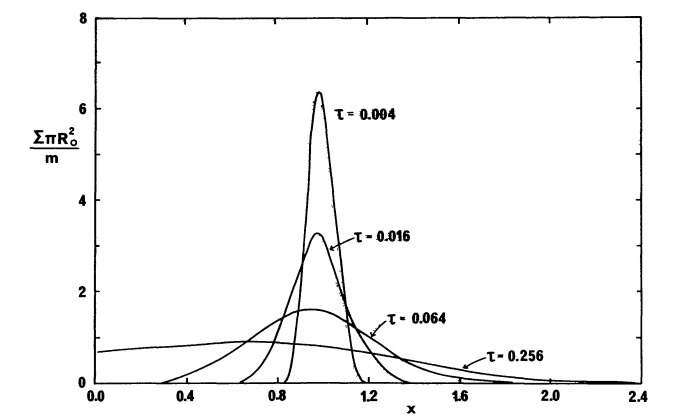
\includegraphics[width=0.7\linewidth]{DensSuper}
		\caption{Evoluzione viscosa di un disco di materia di massa $m$ in funzione di $x=R/R_{circ}$, con $\tau=12\nu t/R_{circ}^2$. Immagine da ~\cite{Pringle1981}}
		\label{fig:denssuper}
	\end{figure}
		
	Sempre con l'analogia dell'attrito viscoso fra gli strati del disco, si può ricavare una formula per la \textit{frazione di energia dissipata} per unità di area:
	\begin{equation}
		D(R)=\frac{G\Sigma'}{4\pi R}=\frac{1}{2}\nu\Sigma(R\Omega')^2
	\end{equation}
	Funzione sempre positiva o nulla, nel caso della rotazione rigida, legata ovviamente all'efficacia radiativa $\eta$ del nostro sistema.
	
	La formula di $D(R)$ si ricava considerando i due momenti torcenti che agiscono ai due lati di un anello di gas che si estende tra $R$ e $R+dR$, tali per cui, se vengono divisi per la velocità angolare
	\begin{equation}
		\frac{1}{\Omega}(G(R+dR)-G(R))=\frac{1}{\Omega}\frac{\partial G}{\partial R}dR=\frac{1}{\Omega}\left[\frac{\partial}{\partial R}(G\Omega)-G\Omega'\right]dR
	\end{equation}
	Quest'equazione è formata da due termini, primo dei quali è $\frac{\partial}{\partial R}(G\Omega)dR$, che rappresenta il tasso di "spostamento" dell'energia nel gas per mezzo dei momenti torcenti e se integrato per tutti i raggi ha un valore che dipende solo dalle condizioni agli estremi del disco. Il secondo termine è $-G\Omega'dR$ e rappresenta un tasso di perdita locale di energia meccanica nel gas, che sarà quindi dissipata sotto forma di calore.
	
	La formula di $D(R)$ si ricava considerando che il calore sarà irradiato su entrambe le facce del disco, con superficie $4\pi RdR$.

\newpage
\section{Modello Stazionario di Disco} 	
\subsection{Spettro di emissione}
\subsection{Shakura e Sunyaev}
\newpage
\section{Evoluzione temporale dei dischi e instabilità}
\subsection{La derivazione di Lightman e Eardley}
\subsection{Instabilità termica e viscosa}
\subsection{Considerazioni sull'espressione della viscosità}
\subsection{Spettro di emissione}
\newpage
\section{Conclusioni}

\newpage
\renewcommand{\bibpreamble}{Per regioni di coerenza interna al testo e di visione ordinata degli argomenti, ho cercato di affrontarli seguendo il più delle volte la traccia e le argomentazioni come sono presentatate sul testo di \textit{Frank, King e Raine}~\cite{FrankKingRaineAccretionPower}, manuale di riferimento per quanto riguarda le teorie dell'accrescimento.
	
	Sono stati fondamentali anche alcune  \textit{review} di \textit{King}~\cite{King2012} e \textit{Pringle}~\cite{Pringle1981}, che sintetizzano efficacemente l'argomento dell'accrescimento e permettono di avere una visione di insieme dei risultati ottenuti.
	
	E' stato fondamentale per la mia comprensione dello sviluppo delle teorie, l'analisi e la lettura degli articoli originali sui modelli di disco di accrescimento intorno ai corpi compatti.
	Ho lavorato quindi anche con gli articoli seminali di \textit{Pringle}, \textit{Reese}, \textit{Shakura}, \textit{Sunyaev} e \textit{Pacholczyk}~\cite{PringleReese1972}~\cite{PringleReesePacholczyk1973}~\cite{ShakuraSunyaev1973} e la splendida analisi del lavoro nella fondazione della teoria di accrescimento di Zeldovich svolta da Shakura quest'anno~\cite{ShakuraZeldovich2018}.
	
	Per quanto riguarda in particolare l'argomento della tesi, ovvero l'instabilità nelle regioni dominate dalla pressione radiativa nel modello del disco di accrescimento, ho fatto riferimento al primissimo lavoro a riguardo di \textit{Lightman} ed \textit{Eardley}~\cite{LightmanEardley1974} e ad articoli successivi che estendono, propongono alternative, ne analizzanoi risultati o li computano. Questi sono stati scritti da \textit{Shakura} e \textit{Sunyaev}~\cite{ShakuraSunyaev1976}, \textit{Shapiro} con gli stessi \textit{Lightman} ed \textit{Eardley}~\cite{ShapiroLightmanEardley1976}, \textit{Taam} e \textit{Lin}~\cite{TaamLin1984} e \textit{Teresi}, \textit{Molteni} e \textit{Toscano}~\cite{TeresiMolteniToscano2004}.
	
	Per tutti gli aspetti non strettamente legati all'accrescimento ho fatto riferimento a tre manuali: il \textit{Maoz}~\cite{MaozNutshell} e il \textit{Prialnik} ~\cite{PrialnikStellarStructureEvolution} per i cenni sulla struttura dei corpi compatti e il \textit{Ghisellini}~\cite{GhiselliniRadiativi} per quanto riguarda i processi radiativi.}

\begin{thebibliography}{9}
	\bibitem{FrankKingRaineAccretionPower} 
	J. Frank, A. King, D. Raine
	"Accretion Power in Astrophysics"\\
	\textit{Cambridge University Press}, 2002 (III ed.)
	
	\bibitem{King2012} 
	A. King 
	"Accretion Disc Theory since Shakura and Sunyaev"\\
	\textit{arXiv}: 1201.2060v1\\
	\textit{to appear in proceedings of 'The Golden Age of Cataclysmic Variables', Memorie Società Astronomica Italiana, 2012 (F. Giovannelli and L. Sabau-Graziati eds.)}
	
	\bibitem{GhiselliniRadiativi} 
	G. Ghisellini
	"Radiative Processes in High Energy Astrophysics"\\
	\textit{Springer}, 2013
	
	\bibitem{LightmanEardley1974} 
	A. P. Lightman, D. M. Eardley 
	"Black Holes in Binary Systems: Instability of Fisk Accretion"\\
	\textit{Astrop. Journal} 187, L1-L3, 1974 January 1
	
	\bibitem{MaozNutshell} 
	D. Maoz
	"Astrophysics in a nutshell"\\
	\textit{Princeton University Press}, 2007
	
	\bibitem{PrialnikStellarStructureEvolution} 
	D. Prialnik
	"An Introduction to the Theory of Stellar Structure and Evolution"\\
	\textit{Cambridge University Press}, 2000
	
	\bibitem{Pringle1981} 
	J. E. Pringle 
	"Accretion Discs in Astrophysics"\\
	\textit{Ann. Rev. Astron. Astrphys.} 1981, 19:137-62
	
	\bibitem{PringleReese1972} 
	J. E. Pringle, M. J. Rees
	"Accretion Discs Model for Compact X-Ray Sources"\\
	\textit{Astron. \& Astrphys.} 21, 1-9 (1972)
	
	\bibitem{PringleReesePacholczyk1973} 
	J. E. Pringle, M. J. Rees, A. G. Pacholczyk
	"Accretion onto Massive Black Holes"\\
	\textit{Astron. \& Astrphys.} 29, 179-184 (1973)
	
	\bibitem{ShakuraSunyaev1973}
	N. I. Shakura, R. A. Sumyaev 
	"Black Holes in Binary Systems. Observational Appearance"\\
	\textit{Astron. \& Astrophys.} 24, 337-355 (1973)
	
	\bibitem{ShakuraSunyaev1976}
	N. I. Shakura, R. A. Sumyaev 
	"A Theory of the Instability of Disk Accretion on to Black Holes and the Variability of Binary X-Ray Sources, Galactic Nuclei and Quasars"\\
	\textit{Mon. Not. R. astr. Soc.} (1976) 175, 613-632
	
	\bibitem{ShakuraZeldovich2018}
	N. I. Shakura
	"Ya. B. Zeldovich and foundation of the accretion theory"\\
	\textit{arXiv}: 1809.1137v1
	
	\bibitem{ShapiroLightmanEardley1976} 
	S. L. Shapiro, A. P. Lightman, D. M. Eardley 
	"A Two-Temperature Disk Model for Cygnus X-1 Structure and Spectrum"\\
	\textit{Astrop. Journal} 187-199, 1976 February 15
	
	\bibitem{TaamLin1984} 
	R. E. Taam, D. N. C. Lin 
	"The Evolution of the Inner Regions of Viscous Accretion Disks Surrounding Neutron Stars"\\
	\textit{Astrop. Journal} 287, 761-768 1984 December 15
	
	\bibitem{TeresiMolteniToscano2004} 
	V. Teresi, D. Molteni, E. Toscano 
	"SPH Simulations of Shakura-Sunyaev Instability at Intermediate Accretion Rates"\\
	\textit{Mon. Not. R. Astron. Soc.} 348, 361-367 (2004)
\end{thebibliography}

\end{document}
